% !Tex program = pdflatex

\documentclass[UTF8]{ctexart}
\CTEXsetup[format={\Large\bfseries}]{section}
\usepackage{amsmath}
\usepackage{amssymb}
\usepackage{ctex}
\usepackage{array}
\usepackage{ulem}
\usepackage{graphicx}
\usepackage{booktabs}
\usepackage{listings}
\usepackage{xcolor}
\usepackage{geometry}
\usepackage{multirow}
\usepackage{subfig}
\usepackage{float}
\usepackage{multicol}
\usepackage{multirow}
\usepackage{pgfplots}
\pgfplotsset{compat=1.16}
\usepackage{diagbox}
\usepackage{indentfirst}
\setlength {\parindent} {2em} 
% small vertical space between paragraphs for readability
\setlength{\parskip}{0.6em}
\usepackage{makecell}
\geometry{papersize={21cm,29.7cm}}
\geometry{left=2.54cm,right=2.54cm,top=3.18cm,bottom=3.18cm}
\usepackage{fancyhdr}
\pagestyle{fancy}
\lhead{\today}
\chead{}
\rhead{2023012274}
\lfoot{清华大学}
\cfoot{\thepage}
\rfoot{模式识别与机器学习}
\renewcommand{\headrulewidth}{0.4pt}
\renewcommand{\headwidth}{\textwidth}
\renewcommand{\footrulewidth}{0pt}
\usepackage{bm}
% listings style for code snippets
\lstset{
    backgroundcolor=\color{white},
    basicstyle=\ttfamily\small,
    breaklines=true,
    framesep=4pt,
    frame=single,
    rulecolor=\color{gray!40},
    keywordstyle=\color{blue},
    commentstyle=\color{gray!60}\itshape,
    showstringspaces=false,
}

\begin{document}
\begin{titlepage}
     \begin{center}
        \quad \\
        \quad \\
        \quad \\
        \quad \\
        \quad \\
        \quad \\
        \quad \\
        \quad \\ 
        \quad \\ 
        {\kaishu \fontsize{30}{15}\selectfont 《模式识别与机器学习》}\\
        \quad \\
        \quad \\
        {\kaishu \fontsize{30}{15}\selectfont 大作业：图像分类}\\

        \end{center}
        \vskip 8cm

        \begin{center}
        \begin{large}
        \begin{tabular}{cc}
        院\qquad 系:& ~~~~~~~~自动化系~~~~~~~~      \\
        \cline{2-2}\\
        班\qquad 级:& 自31班   \\
        \cline{2-2}\\
        学生姓名:& 苟左    \\
        \cline{2-2}\\
        学\qquad 号:&2023012274   \\
        \cline{2-2}
          \end{tabular}
        \end{large}
      \end{center}

\end{titlepage}
\newpage

\section{实验目的}
\begin{enumerate}
    \item 掌握传统模式识别方法在图像分类任务中的应用，理解特征提取与分类器设计的基本流程。
    \item 掌握深度学习方法在图像分类任务中的应用，理解端到端的模型训练、优化与推理过程。
    \item 对比分析传统方法与深度学习方法在 CUB-200 鸟类数据集上的性能差异，深入理解不同方法的优缺点及适用场景。
    \item 提升代码实践能力，包括数据集加载、模型构建、训练循环实现及结果评估等。
\end{enumerate}

\section{实验任务与方法}

\subsection{数据集}
本实验使用 \textbf{CUB-200 鸟类数据集}：
\begin{itemize}
    \item \textbf{数据描述}：共包含 200 个鸟类类别，每个类别约 60 个样本。
    \item \textbf{数据划分}：按照 9:1 的比例划分为训练集和测试集。
    \item \textbf{数据形式}：对于每个样本，提供原始 RGB 图像（用于深度学习任务）和对应的特征向量（用于传统方法任务）。
\end{itemize}

\subsection{任务 1：传统模式识别方法}
\subsubsection{任务描述}
从给定的 200 类样本中随机选取 10 类，利用提供的特征向量完成 10 分类任务。

\subsubsection{方法设计}
\begin{itemize}
    \item \textbf{特征数据}：直接使用数据集提供的 `.pt` 特征文件。
    \item \textbf{分类器设计}：基于课上提到的 \textbf{一对多(One-vs-Rest)} 策略的多分类 SVM。
    \begin{itemize}
        \item \textbf{策略}：对于 $K$ 个类别，训练 $K$ 个二分类 SVM。第 $i$ 个 SVM 将第 $i$ 类样本作为正例（+1），其余所有类别样本作为负例（-1）。
        \item \textbf{求解}：利用 `sklearn.svm.SVC` 求解每个二分类任务的对偶优化问题。
        \item \textbf{预测}：对于测试样本，计算其在 $K$ 个分类器上的决策函数值（即到超平面的距离），选择数值最大的类别作为预测结果。
    \end{itemize}
    \item \textbf{数据预处理}：使用 `StandardScaler` 对特征向量进行标准化处理。
\end{itemize}

\subsection{任务 2：深度神经网络方法}
\subsubsection{任务描述}
使用原始 RGB 图片作为输入，从头开始训练一个深度神经网络，完成 200 类的全分类任务，不使用预训练权重。

\subsubsection{方法设计}
\begin{itemize}
    \item \textbf{模型架构}：考虑到浅层 CNN 难以满足 CUB-200 细粒度分类的需求，通过查阅资料，选择采用更深、更强大的 \textbf{ResNet-18} 架构。
    \begin{itemize}
        \item \textbf{残差结构}：网络由一系列残差块（BasicBlock）组成，每个块包含两个 $3 \times 3$ 卷积层和跳跃连接（Shortcut Connection）。这种结构能有效缓解深层网络中的梯度消失问题，使得训练更深的网络成为可能。
        \item \textbf{网络层级}：包含 4 个残差阶段（Stage），通道数分别为 64, 128, 256, 512。最后通过全局平均池化（Global Average Pooling）和全连接层输出 200 个类别的预测。
    \end{itemize}
    \item \textbf{数据增强}：由于训练样本较少（每类约 60 张），容易导致过拟合，考虑实施课上提到的部分数据增强策略：
    \begin{itemize}
        \item \textbf{随机裁剪}：先将图片放大至 256，再随机裁剪出 224 的区域。
        \item \textbf{随机旋转}：在 $\pm 15^\circ$ 范围内随机旋转图片。
        \item \textbf{颜色抖动}：随机调整亮度、对比度和饱和度，模拟不同光照条件。
        \item \textbf{水平翻转}：随机水平翻转图片。
    \end{itemize}
    \item \textbf{训练策略}：
    \begin{itemize}
        \item \textbf{优化器}：使用 Adam 优化器，初始学习率 0.001，并引入权重衰减（衰减率 $1 \times 10^{-4}$）以正则化模型参数。
        \item \textbf{学习率调度}：采用 `StepLR` 策略，每 10 个 Epoch 将学习率衰减为原来的 0.1，以在训练后期进行更精细的权重更新。
        \item \textbf{训练轮数}：将训练轮数设置为 80 个Epochs，确保模型充分收敛。
    \end{itemize}
\end{itemize}

\section{实验实现与代码片段}

\subsection{任务 1：传统方法实现}

\subsubsection{数据加载}
读取指定类别的 `.pt` 特征文件，并将其转换为 Numpy 数组。

\begin{lstlisting}[language=Python, caption=传统方法数据加载]
def load_data(data_root, split='train', num_classes=10, selected_classes=None):
    split_dir = os.path.join(data_root, split)
    all_classes = sorted([d for d in os.listdir(split_dir) if os.path.isdir(os.path.join(split_dir, d))])

    if selected_classes is None:
        random.seed(42)
        k = min(num_classes, len(all_classes))
        selected_classes = sorted(random.sample(all_classes, k))
    
    # ... (省略中间变量初始化)
    
    for cls_name in selected_classes:
        cls_dir = os.path.join(split_dir, cls_name)
        cls_idx = class_to_idx[cls_name]
        
        for fname in os.listdir(cls_dir):
            if fname.endswith('.pt'):
                fpath = os.path.join(cls_dir, fname)
                feat = torch.load(fpath)
                if isinstance(feat, torch.Tensor):
                    feat = feat.numpy().flatten()
                features.append(feat)
                labels.append(cls_idx)
                    
    return np.array(features), np.array(labels), selected_classes
\end{lstlisting}

\subsubsection{模型训练与预测}
 One-vs-Rest 多分类策略，调用库函数求解二分类 SVM 的优化问题。

\begin{lstlisting}[language=Python, caption=多分类 SVM 实现]
class MulticlassSVM:
    def __init__(self):
        self.classifiers = []
        self.scaler = StandardScaler()

    def train(self, X, y):
        X_scaled = self.scaler.fit_transform(X)
        self.classes = np.unique(y)
        
        # One-vs-Rest 策略：训练 K 个二分类器
        for cls in self.classes:
            # 构建二分类标签：当前类为 1，其他类为 -1
            y_binary = np.where(y == cls, 1, -1)
            
            # 调用库函数求解对偶问题
            clf = SVC(kernel='linear', random_state=42)
            clf.fit(X_scaled, y_binary)
            self.classifiers.append(clf)
            
    def predict(self, X):
        X_scaled = self.scaler.transform(X)
        scores = np.zeros((X.shape[0], len(self.classes)))
        
        # 获取每个分类器的置信度分数
        for i, clf in enumerate(self.classifiers):
            scores[:, i] = clf.decision_function(X_scaled)
            
        # 选择分数最高的类别
        return self.classes[np.argmax(scores, axis=1)]
\end{lstlisting}

\subsection{任务 2：深度学习方法实现}

\subsubsection{数据集类定义}
继承 `torch.utils.data.Dataset`，实现图片的读取和预处理。

\begin{lstlisting}[language=Python, caption=BirdDataset 实现]
class BirdDataset(Dataset):
    def __getitem__(self, idx):
        img_path, label = self.samples[idx]
        image = Image.open(img_path).convert('RGB')
        if self.transform:
            image = self.transform(image)
            
        return image, label
\end{lstlisting}

\subsubsection{ResNet18 网络结构}

\begin{lstlisting}[language=Python, caption=ResNet18 关键实现代码]
import torch
import torch.nn as nn
import torch.nn.functional as F

class BasicBlock(nn.Module):
    expansion = 1
    def __init__(self, in_planes, planes, stride=1):
        super(BasicBlock, self).__init__()
        self.conv1 = nn.Conv2d(in_planes, planes, kernel_size=3, stride=stride, padding=1, bias=False)
        self.bn1 = nn.BatchNorm2d(planes)
        self.conv2 = nn.Conv2d(planes, planes, kernel_size=3, stride=1, padding=1, bias=False)
        self.bn2 = nn.BatchNorm2d(planes)
        self.shortcut = nn.Sequential()
        if stride != 1 or in_planes != self.expansion*planes:
            self.shortcut = nn.Sequential(
                nn.Conv2d(in_planes, self.expansion*planes, kernel_size=1, stride=stride, bias=False),
                nn.BatchNorm2d(self.expansion*planes)
            )
    def forward(self, x):
        out = F.relu(self.bn1(self.conv1(x)))
        out = self.bn2(self.conv2(out))
        out += self.shortcut(x)
        out = F.relu(out)
        return out

class ResNet(nn.Module):
    def __init__(self, block, num_blocks, num_classes=200):
        super(ResNet, self).__init__()
        self.in_planes = 64
        self.conv1 = nn.Conv2d(3, 64, kernel_size=7, stride=2, padding=3, bias=False)
        self.bn1 = nn.BatchNorm2d(64)
        self.layer1 = self._make_layer(block, 64, num_blocks[0], stride=1)
        self.layer2 = self._make_layer(block, 128, num_blocks[1], stride=2)
        self.layer3 = self._make_layer(block, 256, num_blocks[2], stride=2)
        self.layer4 = self._make_layer(block, 512, num_blocks[3], stride=2)
        self.avgpool = nn.AdaptiveAvgPool2d((1, 1))
        self.linear = nn.Linear(512*block.expansion, num_classes)
    def _make_layer(self, block, planes, num_blocks, stride):
        strides = [stride] + [1]*(num_blocks-1)
        layers = []
        for stride in strides:
            layers.append(block(self.in_planes, planes, stride))
            self.in_planes = planes * block.expansion
        return nn.Sequential(*layers)
    def forward(self, x):
        out = F.relu(self.bn1(self.conv1(x)))
        out = F.max_pool2d(out, kernel_size=3, stride=2, padding=1)
        out = self.layer1(out)
        out = self.layer2(out)
        out = self.layer3(out)
        out = self.layer4(out)
        out = self.avgpool(out)
        out = torch.flatten(out, 1)
        out = self.linear(out)
        return out

def ResNet18(num_classes=200):
    return ResNet(BasicBlock, [2, 2, 2, 2], num_classes=num_classes)
\end{lstlisting}

\subsubsection{训练循环}
每个 Epoch 进行一次训练和验证，并记录最佳模型。

\begin{lstlisting}[language=Python, caption=训练主循环]
    for epoch in range(args.epochs):
        print(f"\nEpoch {epoch+1}/{args.epochs}")
        
        train_loss, train_acc = train_one_epoch(model, train_loader, criterion, optimizer, args.device)
        val_loss, val_acc = validate(model, val_loader, criterion, args.device)
        
        print(f"Train Loss: {train_loss:.4f}, Train Acc: {train_acc:.2f}%")
        print(f"Val Loss: {val_loss:.4f}, Val Acc: {val_acc:.2f}%")
        
        if val_acc > best_acc:
            best_acc = val_acc
            torch.save(model.state_dict(), 'best_model.pth')
            print("Saved best model.")
\end{lstlisting}

\section{实验结果与分析}

\subsection{任务 1 结果}
在随机选取的 10 个类别上，使用线性 SVM 进行分类。

\begin{figure}
    \centering
    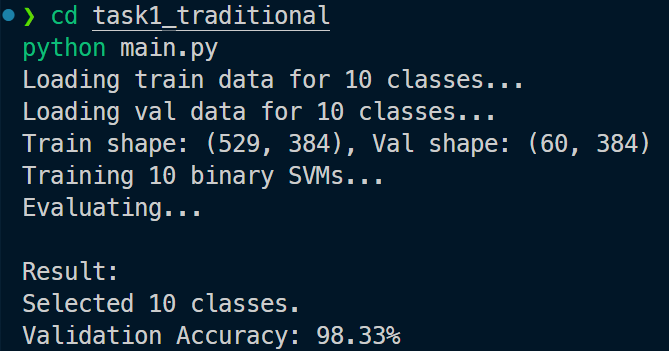
\includegraphics[width=0.7\textwidth]{task1_terminal_output.png}
    \caption{传统方法终端输出}
\end{figure}

\begin{itemize}
    \item \textbf{运行结果}：经过训练，模型在验证集上取得了 \textbf{98.33\%} 的准确率。
    \item \textbf{分析}：
    \begin{itemize}
        \item \textbf{高准确率原因}：提供的特征向量（`.pt` 文件）很可能来自于在大规模数据集（如 ImageNet）上预训练过的深度神经网络（如 ResNet 或 ViT）。这些特征已经包含了极具判别力的高层语义信息，因此即使是简单的线性分类器也能轻松区分不同类别的鸟类。
        \item \textbf{计算效率}：传统方法的训练和推理速度极快，仅需几秒钟即可完成。
    \end{itemize}
\end{itemize}

\subsection{任务 2 结果}

在 200 个类别上，从头训练 ResNet-18 模型（训练 80 个 Epoch）。

\begin{itemize}
    \item \textbf{训练过程及准确率变化情况}：
    下表列出了部分关键 Epoch 的训练准确率（Train Acc）和验证准确率（Val Acc）：
    \begin{table}[H]
    \centering
    \begin{tabular}{cccc}
        \toprule
        Epoch & Train Acc (\%) & Val Acc (\%) & Learning Rate \\
        \midrule
        1   & 1.17  & 2.10  & 0.001000 \\
        5   & 9.53  & 10.16 & 0.001000 \\
        10  & 28.61 & 21.24 & 0.001000 \\
        11  & 40.84 & 38.04 & 0.000100 \\
        15  & 49.49 & 43.07 & 0.000100 \\
        20  & 57.18 & 47.10 & 0.000100 \\
        21  & 60.03 & 48.11 & 0.000010 \\
        27  & 62.22 & 49.29 & 0.000010 \\
        34  & 63.79 & 49.54 & 0.000001 \\
        44  & 63.74 & 49.71 & 0.000000 \\
        61  & 62.95 & 49.87 & 0.000000 \\
        77  & 63.60 & 49.29 & 0.000000 \\
        \bottomrule
    \end{tabular}
    \caption{ResNet-18 训练与验证准确率变化（部分 Epoch）}
    \end{table}

    下图绘制了训练准确率、验证准确率以及学习率随 Epoch 变化的曲线。

    \begin{figure}[H]
    \centering
    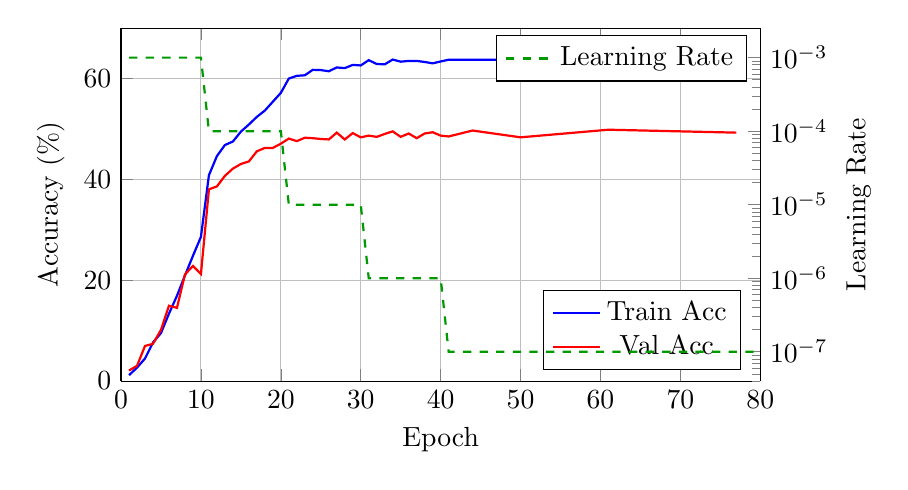
\begin{tikzpicture}
    \begin{axis}[
        xlabel={Epoch},
        ylabel={Accuracy (\%)},
        xmin=0, xmax=80,
        ymin=0, ymax=70,
        axis y line*=left,
        legend pos=south east,
        grid=major,
        width=0.8\textwidth,
        height=0.5\textwidth
    ]
    \addplot[color=blue, mark=none, thick] coordinates {
        (1, 1.17)(2, 2.66)(3, 4.48)(4, 7.65)(5, 9.53)(6, 13.37)(7, 16.92)(8, 20.93)(9, 24.85)(10, 28.61)
        (11, 40.84)(12, 44.64)(13, 46.83)(14, 47.53)(15, 49.49)(16, 50.90)(17, 52.42)(18, 53.67)(19, 55.43)(20, 57.18)
        (21, 60.03)(22, 60.56)(23, 60.67)(24, 61.75)(25, 61.70)(26, 61.47)(27, 62.22)(28, 62.09)(29, 62.73)(30, 62.62)
        (31, 63.67)(32, 62.91)(33, 62.84)(34, 63.79)(35, 63.37)(36, 63.52)(37, 63.52)(38, 63.31)(39, 63.04)(40, 63.41)
        (41, 63.76)(44, 63.74)(50, 63.73)(61, 62.95)(77, 63.60)
    };
    \addlegendentry{Train Acc}

    \addplot[color=red, mark=none, thick] coordinates {
        (1, 2.10)(2, 3.02)(3, 6.97)(4, 7.39)(5, 10.16)(6, 14.95)(7, 14.53)(8, 21.16)(9, 22.84)(10, 21.24)
        (11, 38.04)(12, 38.62)(13, 40.72)(14, 42.15)(15, 43.07)(16, 43.58)(17, 45.59)(18, 46.26)(19, 46.26)(20, 47.10)
        (21, 48.11)(22, 47.61)(23, 48.28)(24, 48.19)(25, 48.03)(26, 47.94)(27, 49.29)(28, 47.94)(29, 49.20)(30, 48.36)
        (31, 48.70)(32, 48.45)(33, 49.03)(34, 49.54)(35, 48.45)(36, 49.12)(37, 48.19)(38, 49.12)(39, 49.37)(40, 48.70)
        (41, 48.53)(44, 49.71)(50, 48.36)(61, 49.87)(77, 49.29)
    };
    \addlegendentry{Val Acc}
    \end{axis}

    \begin{axis}[
        ylabel={Learning Rate},
        xmin=0, xmax=80,
        ymode=log,
        axis y line*=right,
        axis x line=none,
        width=0.8\textwidth,
        height=0.5\textwidth,
        ylabel near ticks
    ]
    \addplot[color=green!60!black, mark=none, dashed, thick] coordinates {
        (1, 0.001)(10, 0.001)
        (11, 0.0001)(20, 0.0001)
        (21, 0.00001)(30, 0.00001)
        (31, 0.000001)(40, 0.000001)
        (41, 0.0000001)(80, 0.0000001)
    };
    \addlegendentry{Learning Rate}
    \end{axis}
    \end{tikzpicture}
    \caption{ResNet-18 训练过程训练准确率、验证准确率与学习率的变化曲线}
    \label{fig:resnet_training}
    \end{figure}

    可以看到，训练准确率从初期的 1.17\% 快速提升至 60\% 以上，验证准确率则在 49\% 左右达到瓶颈，反映出模型在小样本细粒度任务中的泛化能力有限。
    \item \textbf{最终性能}：
    最佳训练集准确率约为 \textbf{63.60\%}（Epoch 77），最佳验证集准确率为 \textbf{49.87\%}（Epoch 61）。
    \item \textbf{结果分析}：
    \begin{itemize}
        \item 最开始尝试采用含4个卷积层的浅层 CNN，所得验证准确率极低 (<1\%)；而 ResNet-18 的残差连接成功解决了深层网络的退化问题，使得模型能够提取到更具判别力的细粒度特征。
        \item 在小样本数据集上，强力的数据增强（裁剪、旋转、变色）可以明显扩充了训练数据的多样性，有效抑制过拟合，使得模型在验证集上的表现稳步提升。
        \item 尽管取得了近 50\% 的准确率，但与直接使用预训练特征的传统方法（98\%+）相比仍有差距。对造成这种差异的限制因素分析如下：
        \end{itemize}
        \begin{enumerate}
            \item \textbf{数据量匮乏}：每类仅 60 张图片对于从头训练深度 CNN 来说远远不够，模型难以学习到具有高度泛化能力的特征表示。
            \item \textbf{缺少预训练权重}：现代计算机视觉任务通常依赖于在 ImageNet 等海量数据上预训练的权重，本任务属于“冷启动”，优化难度很大。
        \end{enumerate}
    \end{itemize}
\end{itemize}

\section{实验结论}
分别通过传统方法和深度学习方法实现了图像分类任务，并进行对比研究。结论如下：
\begin{enumerate}
    \item \textbf{传统方法}：基于高质量预提取特征的线性 SVM 展现了极高的效率和准确率（98.33\%），说明在特征工程得当的情况下，传统方法在小样本任务中依然具有明显的优势。
    \item \textbf{深度学习方法}：
    \begin{itemize}
        \item \textbf{挑战}：在禁止预训练和小样本等限制下，从头训练深度模型面临巨大的过拟合风险和优化难度。简单的 CNN 结构几乎无法收敛。
        \item \textbf{解决方案}：通过引入 \textbf{ResNet 残差结构} 和 \textbf{数据增强}，能够获得 \textbf{63.60\%} 的最佳训练准确率和 \textbf{49.87\%} 的最佳验证准确率。
    \end{itemize}
    \item \textbf{方法对比}：传统方法依赖于强大的预训练特征，适合小样本任务，具有高效、准确的优势；而深度学习方法则需要大量数据和计算资源，适合大规模任务。两者各有优劣，选择时需根据具体应用场景权衡。
    \item \textbf{实验收获}：通过本实验，深入理解了传统模式识别与深度学习在图像分类任务中的不同实现路径和性能表现，提升了实际编码和模型训练的能力。
\end{enumerate}

\end{document}
